
\documentclass[fleqn,10pt]{article} % Document font size and equations flushed left


\usepackage{hyperref} % Required for hyperlinks
\usepackage{graphicx}
\usepackage[english]{babel}
\usepackage{caption}
\DeclareGraphicsExtensions{.pdf,.png,.jpg}


\begin{document}

\title{Article Title} % Article title

\author{Tom Newport} % Authors
\maketitle


\begin{abstract}
There's nothing here yet
\end{abstract}

\maketitle % Print the title and abstract box

\tableofcontents % Print the contents section

\thispagestyle{empty} % Removes page numbering from the first page

%----------------------------------------------------------------------------------------
%	ARTICLE CONTENTS
%----------------------------------------------------------------------------------------
% Total word count should be approx. 4500 words

% Add command to format binomial species name:
\newcommand{\bn}
[1]{\textit{#1}}

% Add shortcut for P. falciparum
\newcommand{\pf}
{\bn{P. falciparum }}

% Add semantic strong (replaces bold)
\newcommand{\str}
[1]{\textbf{#1}}

\section{Introduction} 

%% TN Introduce Plasmodium falciparum, establish that it lives inside red blood cells
The apicomplexan parasite \bn{Plasmodium falciparum} is the most virulent causative agent of malaria, and responsible for over 600,000 deaths annually \cite{WorldHealthOrganisation2013}. Along with other members of the \bn{Plasmodium} family, \pf has a complex lifecycle, moving between several different tissues in both mammalian and arthropod hosts. Symptomatic disease in humans occurs when \pf undergoes rounds of asexual reproduction inside human red blood cells (RBCs) \cite{Chen2000}.

%% TN Introduce RBC intracellular environment, benefits and challenges
In some respects, the intracellular environment of a red blood cell is an ideal location for parasite proliferation. The cells' lack of an MHC (Major Histocompatibility Complex) system, which would otherwise be used to identify intracellular pathogens to the host immune system, renders parasites immunologically invisible \cite{Kirchgatter2005}, whilst the vascular system allows the parasite to travel throughout the body. The highly specialised nature of RBCs, however, means that the intracellular environment also presents significant challenges to parasite survival.

%% TN Introduce challenges to pf survival
Mature red blood cells lack protein production and export machinery, and are a nutritionally poor environment, with a proteome dominated by haemoglobin, which typically accounts for around 98\% of the protein content of the cell \cite{DAlessandro2010}. \pf is able to digest RBC proteins, however haemoglobin lacks several amino acids required for protein production. Red blood cells are also  subject to regular 'quality control' in the spleen, where damaged or infected cells are killed and recycled \cite{Elsworth2014}.

%% TN Introduce exportome
In order to survive and proliferate inside RBCs, \pf exports a range of proteins which radically transform the red blood cell, collectively termed the \str{exportome}. Many of these proteins are involved in setting up a parasite-derived protein export system, capable of directing exported \pf proteins to sites both inside and outside the RBC. \pf resides inside a parasitophorous vacuole, and exports proteins via structures termed Maurer's Clefts \cite{Marti2013}, which bear some similarity to golgi apparatus \cite{Mundwiler-Pachlatko2013}.

%% TN Split paragraph
In order to avoid detection in the spleen, many exported proteins are associated with the formation of knobs, specialised structures which form at the RBC membrane and promote cytoadherence to epithelial cells, platelets and other red blood cells \cite{Kraemer2006}. Severe forms of malaria, including cerebral malaria, are believed to be caused by sequestration of infected red blood cells in deep tissues, as well as overinduction of inflammatory cytokines \cite{Chen2000}. Other exported components have been associated with increasing RBC membrane permeability to facilitate nutrient and waste exchange and strengthening the RBC cytoskeleton (Reviewed in \cite{Elsworth2014}). 

%% TN Introduce exportome in a genomic context
To date, at least 10\% of the protein products of the \pf genome have been shown to be exported to the host cell \cite{Boddey2013a}. Within this exportome, there exist 360 distinct proteins once close duplicates are excluded.

%% Why predict the exportome?
Whilst the \pf genome has been available since 2002 \cite{Gardner2002}, comparatively few genes have been studied in depth, and many remain of unknown function. The discovery of a motif termed the PEXEL (Plasmodium Export Element) shared between many exportome components has made it possible to reliably predict the \pf exportome in the absence of other information \cite{Sargeant2006}.

%% The pexel motif, and how this is exported
The PEXEL motif is pentameric, located near the N-terminal of the protein, and can be generalised as the amino acid sequence \texttt{RxLxE/Q/D} \cite{Goldberg2010}, where \texttt{x} is any non-charged amino acid \cite{Dietz2014} although the non-canonical PEXEL motif \texttt{\str{K}xLxE/Q/D} and relaxed PEXEL motif \texttt{Rx\str{x}LxE/Q/D} are also seen occasionally \cite{Elsworth2014}. It is known that the amino acid sequence cleaved after the leucine residue in the parasite ER \cite{Goldberg2010} although how the PEXEL motif targets the protein for export remains unclear. The \pf protein Plasmepsin V has been shown to cleave a subset of PEXEL-carrying proteins \cite{Boddey2013}.

% Possible - Where do pexel proteins go next?

In addition to exported PEXEL proteins, several PEXEL Negative exported proteins have been identified using transcription profiling \cite{Heiber2013}. Based on experimental evidence, a cryptic signal is though to exist near the N-terminal of both mature (cleaved) PEXEL proteins and PNEPs \cite{Gruring2012}, although the nature of this sequence remains unclear.

Understanding the protein-protein interactions responsible for the transformation of the infected red blood cell is both an interesting scientific challenge and an important step towards a better understanding of malaria in humans. Whilst an interactome for \pf proteins has been produced using a yeast-two-hybrid \cite{LaCount2005} it is of low quality and contains many false positives.

\subsection{Protein Structure Prediction}

The design of constructs for experimental use is hampered somewhat a lack of structural information about \pf exportome components. To date, only 4 components of the \pf exportome have solved structures in the PDB (own research, \url{https://gist.github.com/tomnewport/a04868602d3482d33921}), and so knowledge based modelling using a tool such as MODELLER \cite{Eswar2007} is not applicable. There exist several tools, however, which are able to predict features and domains of proteins using a variety of approaches.

\subsubsection*{Secondary Structure and Disorder Prediction}

Parts of a protein such as helices and strands will have a fixed 3D structure and pattern of amino acids and are said to be ordered. Other parts of the protein, especially loops, may not possess such an ordered or fixed structure and so are said to be disordered. Disordered parts of a protein often connect domains or features of the protein secondary structure and so disorder prediction can be used to find domain boundaries. Several algorithms exist to predict both secondary structure and disorder from amino acid sequence, and the tool metaPrDOS \cite{Ishida2008} can be used to obtain a consensus from a selection of disorder prediction algorithms.

\subsubsection*{Coiled Coil Prediction}

Coiled coils are a common structural motif whereby two or more alpha helices are wound together, often important in the formation of obligomers and complexes. The COILS software tool uses a database of known coiled coil motifs to predict the likelihood of a coiled coil at particular sites on in an amino acid sequence \cite{Lupas1991}.

\subsubsection*{Transmembrane Prediction}

Proteins may include several domains which cross or interact with the hydrophobic environment of the lipid membrane of a cell or compartments within the cell. The software tool TMHMM uses a hidden Markov model based approach to predict these domains based on the protein's amino acid sequence alone \cite{Krogh2001}.

\subsubsection*{Combined Approaches}

Some software tools combine several different approaches to structure prediction. InterPro \cite{Mulder2002} performs coiled coil prediction and transmembrane prediction, and searches for known domains with similar sequences. Results are presented in a single graphic showing predicted domains along the amino acid sequence.

Phyre2 \cite{Kelley2009} performs disorder prediction, secondary structure prediction and transmembrane prediction before comparing against a fold database and attempting to build a model of the tertiary structure based on the amino acid sequence. Results are presented in a series of figures as well as 3D models based on different templates in a PDB format.

\section{Software implementation}
\subsection{Aims}

This project aims to build software tools to automate bioinformatic analysis of \pf exported proteins and red blood cell proteins and present the results in a web-based interface. This will be used to aid in the design of protein constructs used to produce a high quality interactome for exported \pf proteins. 

% Shortcomings of existing tools and databases

\begin{figure}
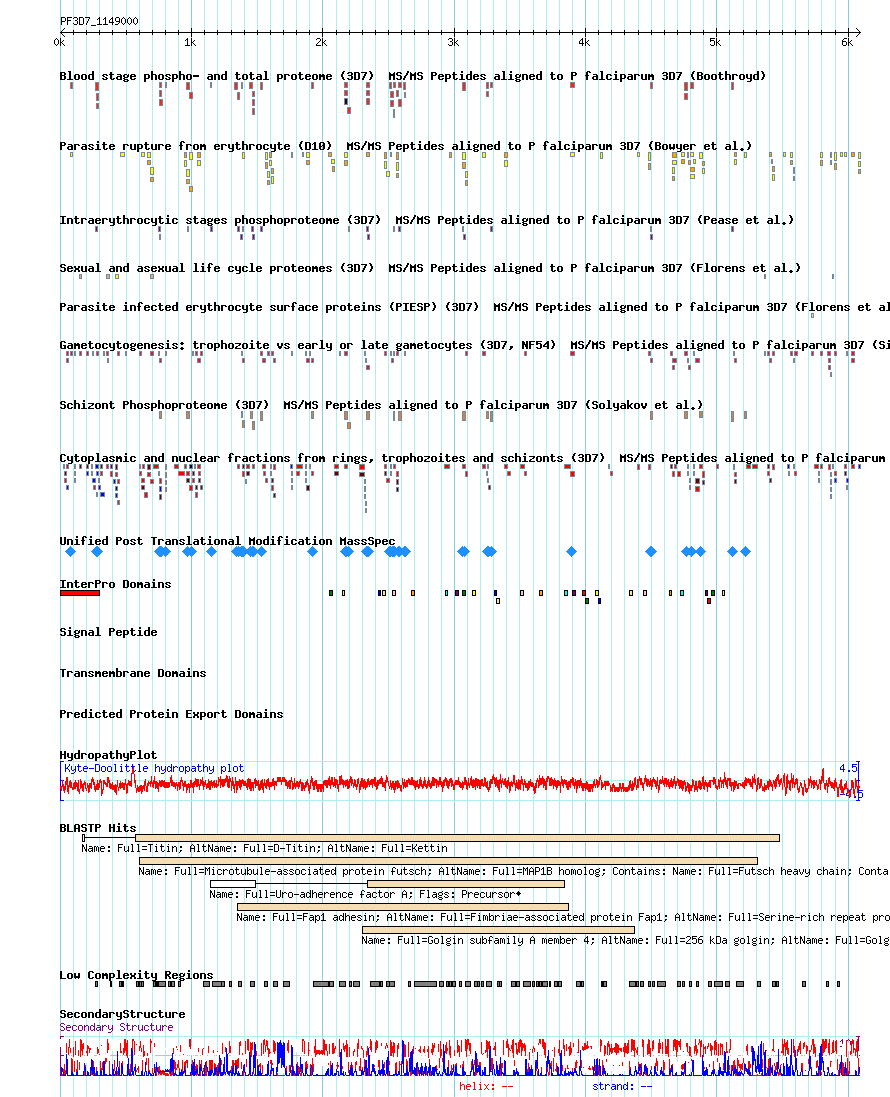
\includegraphics[width=7cm]{figs/plasmodbview}
\caption{\str{PlasmoDB Structural information for PF3D7\_1149000} | This includes, amongst others, InterPro domains, secondary structure prediction and export domains. Note that the protein product of PF3D7\_1149000 has been shown to be exported.}
\end{figure}

The \pf genome and other associated data are already available from several online databases, including the dedicated PlasmoDB (\url{http://plasmodb.org/}) \cite{Aurrecoechea2009} which provides functional genomic data for genes found in several \bn{Plasmodium} species and includes annotations such as gene location, polymorphisms and expression data, as well as some limited structural annotations (Figure 1). No database presently provides a broad range of structural annotations required for construct design, or allows the user to look only at proteins known to be exported to the red blood cell.

% Flexibility and modularity

Protein structure prediction is a fast evolving field. As existing tools are updated and new tools are published, both the inputs and outputs of such a tool may change. It is therefore vital to consider modularity and flexibility at an early stage to ensure future development is not compromised by design decisions made earlier in development.

\subsection{Overview}

\begin{figure}
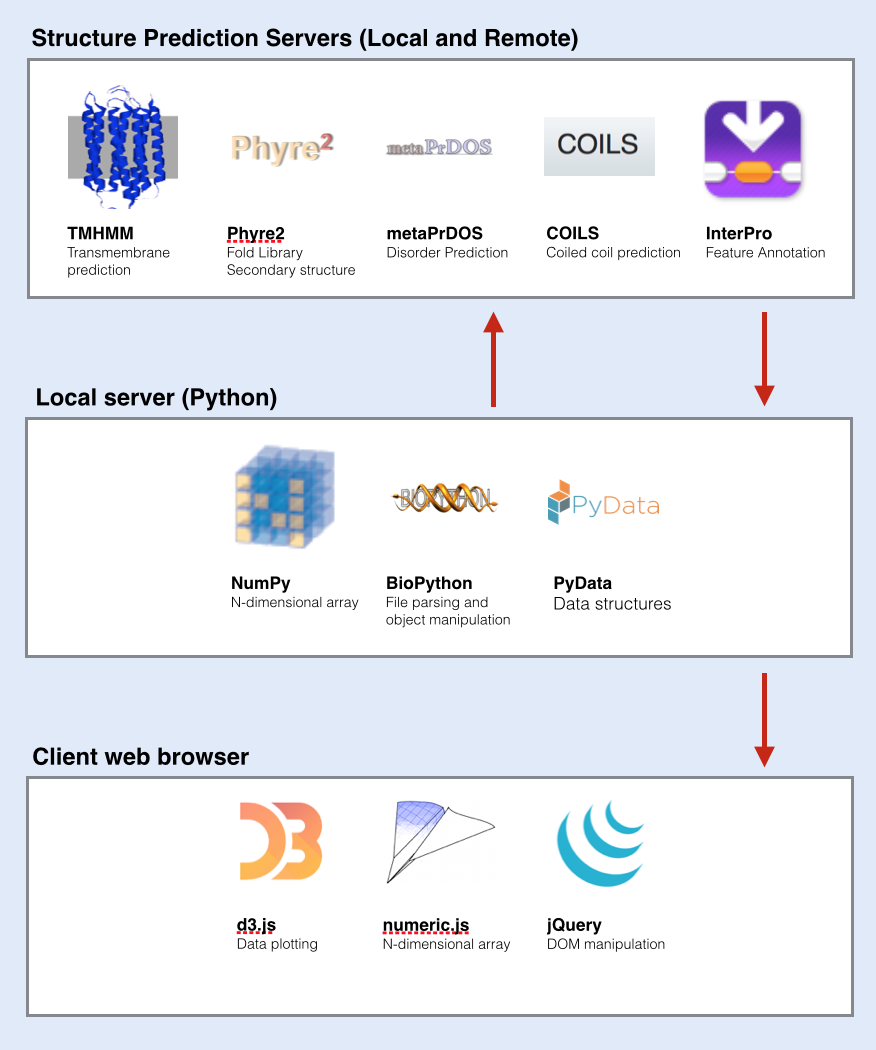
\includegraphics[width=9cm]{figs/softwareoverview}
\caption{\str{High-level overview of planned software} | Sequence data is submitted to the servers TMHMM, Phyre2, metaPrDOS, COILS and InterPro using a python script running on a local server. The data is then retrieved and processed. Once processed and stored, data may be requested by the client and displayed using client-side scripts for visualisation.}
\end{figure}

The finished software will consist of three distinct parts. A local client implemented in Python, will request analyses of newly added sequences from remote servers and then parse and store the response, whilst a remote client implemented in JavaScript will load and display protein files to the end user. A simple HTTP server will serve and cache JavaScript files necessary for the remote client and data files generated by the Python client.

\subsubsection{Python server}

The local python client, which is responsible for requesting, retrieving and parsing structure predictions, may be provided with a list of gene names which correspond to genes available through PlasmoDB (\url{http://plasmodb.org/}) \cite{Aurrecoechea2009}. These will then be retrieved in FASTA format from PlasmoDB and submitted several servers: TMHMM for transmembrane prediction; Phyre2 for fold recognition and secondary structure predication; metaPrDOS for disorder prediction; COILS for coiled coil prediction and InterPro for feature annotation. Submission to web-based servers will be performed using HTTP requests to CGI (Common Gateway Interface) scripts on respective remote servers using the Python Requests library (\url{http://python-requests.org}) and similarly retrieved once completed.

Parsing of results will be performed primarily using the Pandas dataframe provided by PyData (\url{http://pandas.pydata.org}), assisted by BioPython \cite{Cock2009}, used to open files in biological formats such as PDB and FASTA, and Numpy \cite{VanderWalt2011}, which implements a computationally efficient n-dimensional array for the Python language. Results from many servers will be saved to two files in comma-separated values format, one storing series with a defined value for each amino acid (a prediction of the likelihood of each amino acid forming part of a coiled coil, for example), and one (annotations) storing annotations identifying features stretching across several amino acids (domains identified based on similarity to common motifs in a database, for example).

\begin{table}[h]
\begin{tabular}{llllll}
\textbf{Position} & \textbf{Amino Acid} & \textbf{Series 1} & \textbf{Series 2} & \textbf{...} & \textbf{Series N} \\
1                 & S                   & 0.2               & 20                & ...          & 0.9               \\
2                 & N                   & 0.3               & 14                & ...          & 0.1               \\
3                 & I                   & 0.2               & 12                & ...          & 0.3              
\end{tabular}
\caption{\str{Series Table Example} | Each series has a defined value for each amino acid. Each column represents a single series, and the table possesses an unlimited number of columns. Each row represents a single amino acid.}
\end{table}

\begin{table}[h]
\begin{tabular}{llll}
\textbf{Start Position} & \textbf{End Position} & \textbf{Source} & \textbf{Description}       \\
10                      & 143                   & InterPro        & Transmembrane Region       \\
53                      & 197                   & Phyre2          & Duffy receptor, alpha form
\end{tabular}
\caption{\str{Annotation Table Example} | Each annotation consists of a start position and an end position, a source (the server which identified it) and a description (the feature which was identified by the server). Each row is an annotation, and the table may contain an unlimited number of rows.}
\end{table}

\subsubsection{Public facing server}

Since the public-facing HTTP server only retrieves files (and is not able to trigger any additional server-side processing), any expertly built HTTP server may be used without modification, greatly simplifying the problems of installing, maintaining and securing a publicly accessible server on the web.

Unlike most existing web-based tools for viewing genomic data where visualisations are rendered on the server and transmitted as images, visualisations will be rendered client-side based on raw data. Users will therefore require a recently updated web browser in order to view visualisations of data using the remote client. The client-side approach removes the need for the server to render images, reducing load on the server, and also removes the need to transmit images, reducing the load on the network. Additionally, advanced users are able to tweak visualisations as required simply by changing rules in the CSS (Cascading StyleSheet) files supplied with the remote client.

\subsubsection{Remote JavaScript client}

An HTML (HyperText Markup Language) document provided by the server will download the remote client and all dependencies (including default style sheets) to the user's web browser. The remote client will consist of two main classes, a \texttt{data\_manager} class which will load data from the server, perform some client side processing and then provide an object which can be used to retrieve data for plotting, and a \texttt{ui\_bindings} class, which will provide an interface which may be used to create, update and link different UI elements.

\subsubsection{The \texttt{data\_manager} class}

\begin{figure}
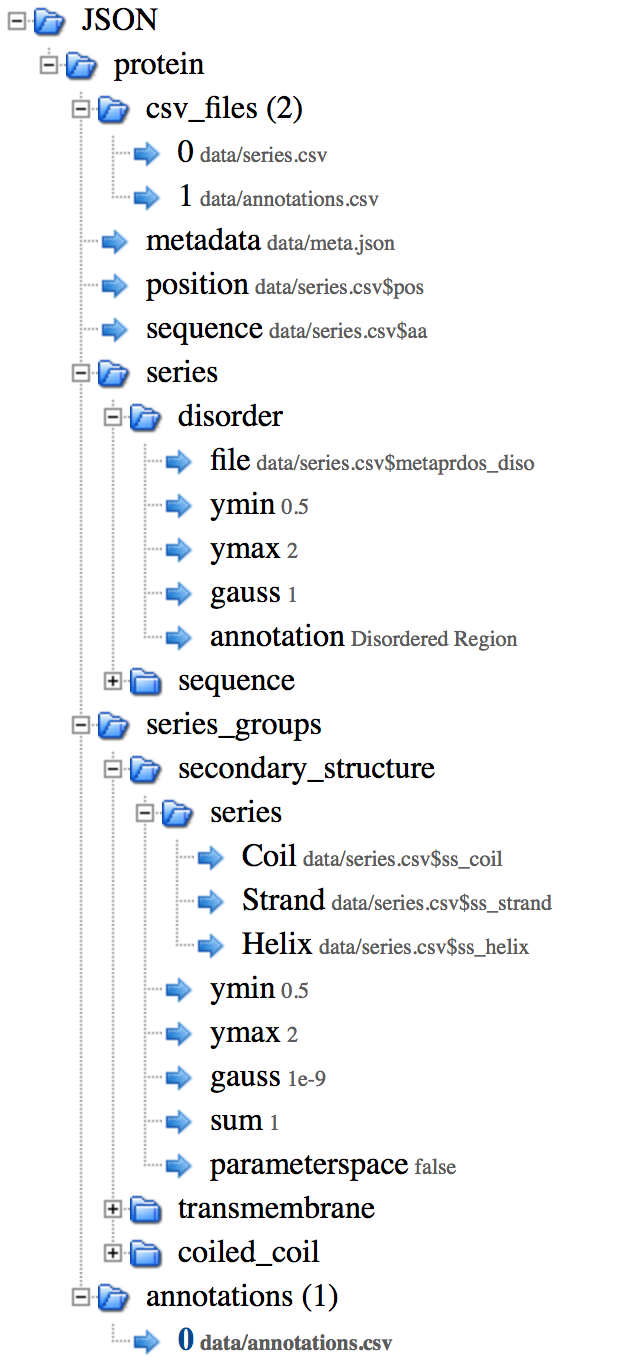
\includegraphics[width=7cm]{figs/schema}
\caption{\str{Tree visualisation of JSON Schema} | Each protein object contains a list of required CSV files and a link to a protein metadata file. Position identifies a spreadsheet column which contains the amino acid position, and sequence identifies a spreadsheet column which contains a single-letter amino acid code for each position. Series are then defined, followed by series groups and finally annotations. Only one object of each type is shown expanded. Visualised using \url{http://www.jsontree.com}.}
\end{figure}

The \texttt{data\_manager} class will first download a schema from the server in JSON format which will describe where data required for visualisations may be found. This will provide a machine readable description of the contents of the data files and the relationships between them. All proteins will likely share a single schema file, however updates to the schema file can be used to change the way the remote client interprets data files. A visualisation of an example schema file is shown in Figure 3. Several objects appear once per schema, including an array of required csv files, a link to protein metadata (properties of the protein such as its length and gene name), an identifier for the position series which contains the position of each amino acid in the series table, and an identifier for the sequence series, which defines the residue at each position.

An unlimited number of three different data types, series, series groups and annotation lists may then be defined.

\paragraph{The \texttt{Series} class}

The series class is named and contains an identifier locating that series within the required csv files. It will also contain minimum and maximum y-value thresholds to annotate features, and the standard deviation of a gaussian kernel convolution kernel which may be used to smooth the series before annotating features, and a description for features annotated in this manner. In the example shown in Figure 3, the named series "disorder" may be convolved using a gaussian kernel of standard deviation 1, and values higher than 0.5 but lower than 2 (unrealistically high to cause upper bound to be ignored) may be annotated as "Disordered Region".

\paragraph{The \texttt{Series\_Group} class}

The series group class is named and contains several series objects. The properties of these objects for annotation are shared, and additional properties may be used to indicate that the series taken together should sum to a particular value for all amino acids, or that the series each represent a different point in parameter space for some algorithm.

\paragraph{The \texttt{Annotation} object}

The annotation object simply contains a list of annotations, with a start, end, source and description. Each protein possesses only one annotation list, which can be populated from multiple files.

\subsubsection{The \texttt{ui\_bindings} class}

The UI Bindings class will consist of a UI Manager, which coordinates initialising and updating UI elements in response to user actions, a viewscope class which defines the part of the sequence being viewed by the user, and a plot class, which keeps an individual plot up to date. Plotting is primarily performed in a vector format using Data Driven Documents (d3.js) \cite{Bostock2011}. 

\paragraph{The UI manager and viewscope}

\paragraph{Plotting}

In the sense used here, a plot may be anything which uses a piece of data to alter the user interface. This may be as simple as printing a piece of text or toggling the visibility of some UI element, or as complex as an interactive visualisation of large amounts of data. The only required feature of a plot is that it should exist at a fixed position in the DOM (Document Object Model) and be able to initialise and update (draw and redraw) itself. Typically plots 'subscribe' to changes in a viewscope object through the UI Manager. For example, a UI element may show disorder in a region of the gene specified by a viewscope object. If the update (redraw) method of the UI element is subscribed to the viewscope object, it will be called each time the user changes the view.

Several different plots will be implemented:

\paragraph{D3 Annotation Plot}
\paragraph{D3 Annotation Plot}
\paragraph{D3 Annotation Plot}
\paragraph{D3 Annotation Plot}



\subsection{Implementation}

% Introduction

% Specific milestones

\section{Discussion}

% Possible overall benefits

% Benefits of flexibility

% Alternatives

\section{Limitations and Further Work}

% Personalised annotations

%300 words
%------------------------------------------------
\phantomsection
\section*{Acknowledgments}

I am grateful to John Vakonakis for his insight, enthusiasm and encouragement whilst supervising this project.

\addcontentsline{toc}{section}{Acknowledgments} % Adds this section to the table of contents

%----------------------------------------------------------------------------------------
%	REFERENCE LIST
%----------------------------------------------------------------------------------------
\phantomsection
\bibliographystyle{unsrt}
\bibliography{references}

%----------------------------------------------------------------------------------------

\end{document}